\documentclass[10pt,a4paper]{article}
\usepackage[utf8]{inputenc}
\usepackage[english]{babel}
\usepackage[left=1.5cm,right=1.5cm,top=1.5cm,bottom=1.5cm]{geometry}
\author{Andreas Hemmetter}
\let\footruleskip\undefined %undefine footruleskip
\usepackage{fancyhdr}
\usepackage{multicol}
% \usepackage{textcomp}
% \usepackage{amsthm}
\usepackage{framed}
\usepackage{multirow}
\usepackage{xhfill}
% \usepackage{bbold}
% \usepackage{amssymb}
\usepackage{hyperref}
\usepackage{booktabs}
\usepackage{graphicx}
%\usepackage{braket}
% \usepackage{tikz}
% \usetikzlibrary{arrows}
\setlength{\headheight}{15.2pt}
\begin{document}
\pagestyle{fancyplain}
\fancyhf{}
\rhead{\textbf{\textit{Toki Pona}} - \href{mailto:a.hemmetter@gmail.com}{A. Hemmetter} }
\rfoot{\scriptsize{This work is licensed under a \href{https://creativecommons.org/licenses/by-sa/4.0/}{Creative Commons Attribution-ShareAlike 4.0 International License}. Image by Bryant Knight (jan Pije).}}
\begin{center}

\begin{tabular}[t]{@{}l}
\rule[4pt]{0.35\linewidth}{4pt}
\end{tabular}
\begin{tabular}[t]{@{}}
\fontsize{24pt}{10pt}
\textbf{Toki Pona}
\end{tabular}
\begin{tabular}[t]{r@{}}
\rule[4pt]{0.35\linewidth}{4pt}
\end{tabular}
\end{center}

\paragraph{What is Toki Pona?}
Toki Pona is a minimalist language, designed by Canadian linguist Sonja Lang to help simplify one's thoughts. It is based on the idea that a small grammar and vocabulary is more than enough for simple communication. Imagine you are stranded on an island with a Babel-esque group of survivors - you can start communicating with nothing more than this piece of paper and a bit of time, which you seem to have a lot of anyway. It's a deliberately simple language, so Keep It Simple, Speaker.

\begin{multicols}{2}
\paragraph{Sounds and Spelling}

Toki Pona uses only sounds that are common to most languages. These are \textbf{k}, \textbf{l}, \textbf{m}, \textbf{n}, \textbf{p}, \textbf{s}, \textbf{t}, \textbf{w} and \textbf{j} (as in \textit{\textbf{y}et}) as consonants and \textbf{a} (\textit{f\textbf{a}ther}), \textbf{e} (\textit{m\textbf{e}t}), \textbf{i} (\textit{p\textbf{ee}l}), \textbf{o} (\textit{\textbf{o}ften}) and \textbf{u} (\textit{f\textbf{oo}d}) as vowels. Possible syllables follow the CV(n) pattern. Words are never capitalized, except for proper names. Due to its limited phonology, Toki Pona can be written in pretty much any writing system, including Hangul, Arabic, Cyrillic and hieroglyphs (\textbf{sitelen suwi} or \textbf{linja pona}). Go wild.

\paragraph{Vocabulary}

Toki Pona has a teeny-tiny vocabulary of 120-ish words and is therefore quite ambiguous. Words are flexible in their gender, number, function in a sentence and even precise meaning.  Essentially, they convey \textit{concepts}, and their function becomes clear from context. For example \textbf{mi moku} can mean \textit{I eat / I will eat / I ate / I am food} etc. You can express more specific words through compound words by adding adjectives \underline{after} the main concept: \textbf{jan} [\textit{person}], \textbf{jan utala} [\textit{fighting person (soldier)}], \textbf{jan utala nasa} [\textit{stupid soldier}], etc. Any word, including \textbf{mute} [\textit{many}], \textbf{ni} [\textit{this}] and the pronouns can act as adjective/adverb after the noun/verb: \textbf{mi utala ike} [\textit{I fight badly}]. A consequential bug (or feature) is that the same thing can be called differently by different people: \textit{coffee} might be \textbf{telo pi lape ala} [\textit{liquid that makes you not sleep}], \textbf{telo wawa pimeja} [\textit{strong black liquid}], \textbf{telo jaki ike} [\textit{disgusting mud-water}], etc. You get the idea.

\paragraph{Sentence Structure}

Go ahead and stick words to each other to express what you want to say. If the sentence becomes too long, split it up or just don't say it. But not so fast! Toki Pona requires identifier \textbf{li} to separate subject and verb (except directly after \textbf{mi} [\textit{I}] and \textbf{sina} [\textit{you}]) and \textbf{e} to separate verb and direct object: \textbf{ona li pona e ilo} [\textit{She fixes the tool}]. Furthermore, multiple \textbf{li} or \textbf{e} can be used as \textit{and}: \textbf{pipi li lukin li moku} [\textit{The bug looks and eats}] and \textbf{mi moku e kili e telo} [\textit{I eat fruit and water}]. There is no \textit{to be}, so \textbf{mi pona} means \textit{I am good}.

\paragraph{Negation and Questions}

A word can be negated by placing \textbf{ala} [\textit{not}] after the verb: \textbf{mi wile ala tawa musi} [\textit{I don't want to dance}]; it essentially acts as an adjective (like also \textbf{ali} [\textit{all}]). Yes/No questions are formed by repeating the verb after \textbf{ala}: \textbf{sina pona ala pona?} [\textit{Are you okay?}]. To answer, repeat the verb with or without \textbf{ala}. To ask for the subject, \textbf{seme} is used: \textbf{seme li lon tomo mi?} [\textit{What is in my house?}]. It can also be used to ask for the direct object (\textbf{sina lukin e seme?} [\textit{What are you watching?}]), the person (\textbf{jan seme li moku?} [\textit{Who is eating?}]), the reason (\textbf{sina kama tan seme?} [\textit{Why did you come?}]) or for a specific thing (\textbf{ma seme li pona tawa sina?} [\textit{Which countries do you like?}]). The word \textbf{anu} [\textit{either/or}] gives a choice between two options: \textbf{sina jo e kili anu telo nasa?} [\textit{Do you have fruit, or is it the wine that you have?}], \textbf{... anu seme?} [\textit{..., or what?}].
\end{multicols}

\paragraph{Prepositions}

Prepositions can also act as verbs, nouns or adjectives - just like any other word - but do not require \textbf{e} before an object. These are \textbf{lon} [\textit{to be in/at something}], \textbf{kepeken} [\textit{to use with something}], \textbf{tawa} [\textit{to move to somewhere}], \textbf{kama} [\textit{to come/cause}], \textbf{sama} [\textit{like}], \textbf{tan} [\textit{because}] and \textbf{poka} [\textit{beside}]. Related to that are modal (helping) verbs such as \textbf{wile} [\textit{want/need}], which can stand right before the predicate (without \textbf{li}).

\begin{multicols}{2}
\noindent\textbf{suno li lon sewi} [\textit{The sun is in the sky}]\\
\noindent\textbf{mi wile e ni: mi lon tomo} [\textit{I want to be at home}]\\
\noindent\textbf{mi tawa tomo mi} [\textit{I am going to my house}]\\
\noindent\textbf{mi toki tawa sina} [\textit{I talk to you}]\\
\noindent\textbf{ni li pona tawa mi} [\textit{That is good for me (I like that)}]\\
\noindent\textbf{mi tawa e kiwen} [\textit{I am moving the rock}]\\
\noindent\textbf{ona li kama tawa tomo mi} [\textit{He came to my house}]\\
\noindent\textbf{mi kama e pakala} [\textit{I caused an accident}]\\
\noindent\textbf{mi kama jo e telo} [\textit{I'm getting water}]\\
\noindent\textbf{mi moku kepeken ilo moku} [\textit{I eat with a fork/spoon}]\\
\noindent\textbf{mi kepeken e poki} [\textit{I use a cup}]\\
\noindent\textbf{mi moku poka jan pona mi} [\textit{I ate beside my friend}]\\
\noindent\textbf{jan ni li sama mi} [\textit{That person is like me}]\\
\noindent\textbf{mi moku tan ni: mi wile moku} [\textit{I eat because I am hungry}]\\
\noindent Other nouns which work as prepositions:\\
\noindent\textbf{ona li lon sewi mi} [\textit{He is above me}]\\
\noindent\textbf{pipi li lon anpa mi} [\textit{The bug is underneath me}]\\
\noindent\textbf{moku li lon insa mi} [\textit{Food is in my stomach}]\\
\noindent\textbf{len li lon poka mi} [\textit{The clothes are at my side}]
\end{multicols}

\paragraph{Things You Don't Need To Say So Accurately}
Colors are given as mixtures/shades of the five basic colors \textbf{jelo} [\textit{yellow}], \textbf{laso} [\textit{blue}], \textbf{loje} [\textit{red}], \textbf{pimeja} [\textit{black}] and \textbf{walo} [\textit{white}]. But don't overdo it: the specific shade of a banana doesn't matter; it's just a \textbf{kili palisa jelo}.\\
\noindent There is no real number system in Toki Pona, since it can almost always be avoided to use concrete, bigger numbers, and because the fun in the language is in the simplification of our thoughts. That being said, it knows four numbers which can be combined to form a few larger ones: \textbf{ala} [\textit{zero}], \textbf{wan} [\textit{one} or \textit{to join}], \textbf{tu} [\textit{two} or \textit{to separate}] and \textbf{luka} [\textit{five}]. These words can be added together to make larger numbers (\textbf{luka tu wan} [\textit{eight}]), but it is advised to use \textbf{mute} [\textit{many}] for everything else. Exact quantities add nothing to the conversation. Try to live without them.\\
If absolutely necessary, tenses can be expressed by \textbf{tenpo pini la ...} (past), \textbf{tenpo ni la ...} (present) and \textbf{tenpo kama la ...} (future), and gender by using the adjectives \textbf{meli} [\textit{female}] and \textbf{mije} [\textit{male}].

\newpage
\paragraph{Details}
\begin{multicols}{2}
\begin{itemize}
\item Country names are always adjectives and follow the syllable formation rules of Toki Pona: \textbf{ma Kanata} [\textit{(the country of) Canada}]. Same goes for languages (\textbf{toki}), nationalities (\textbf{jan}), names (\textbf{jan}), and so on.
\item The imperative is formed by putting an \textbf{o} before the verb: \textbf{o pali!} [\textit{Get to work!}]. People can be addressed by putting an \textbf{o} after their name: \textbf{jan Keli o, sina pona lukin} [\textit{Kelly, you are good-looking}]. When addressing people and commanding them in one sentence, one \textbf{o} can be dropped.
\item The word \textbf{pi} [\textit{of}] separates meanings: \textbf{tomo telo nasa} [\textit{weird bathroom}], \textbf{tomo pi telo nasa} [\textit{house of alcohol (bar)}]. It can also be used to specifify an owner: \textbf{tomo pi jan Lisa} [\textit{Lisa's house}].
\item We can use \textbf{taso} [\textit{so/but/just}] to join related sentences together.
\end{itemize}
\end{multicols}

\begin{center}
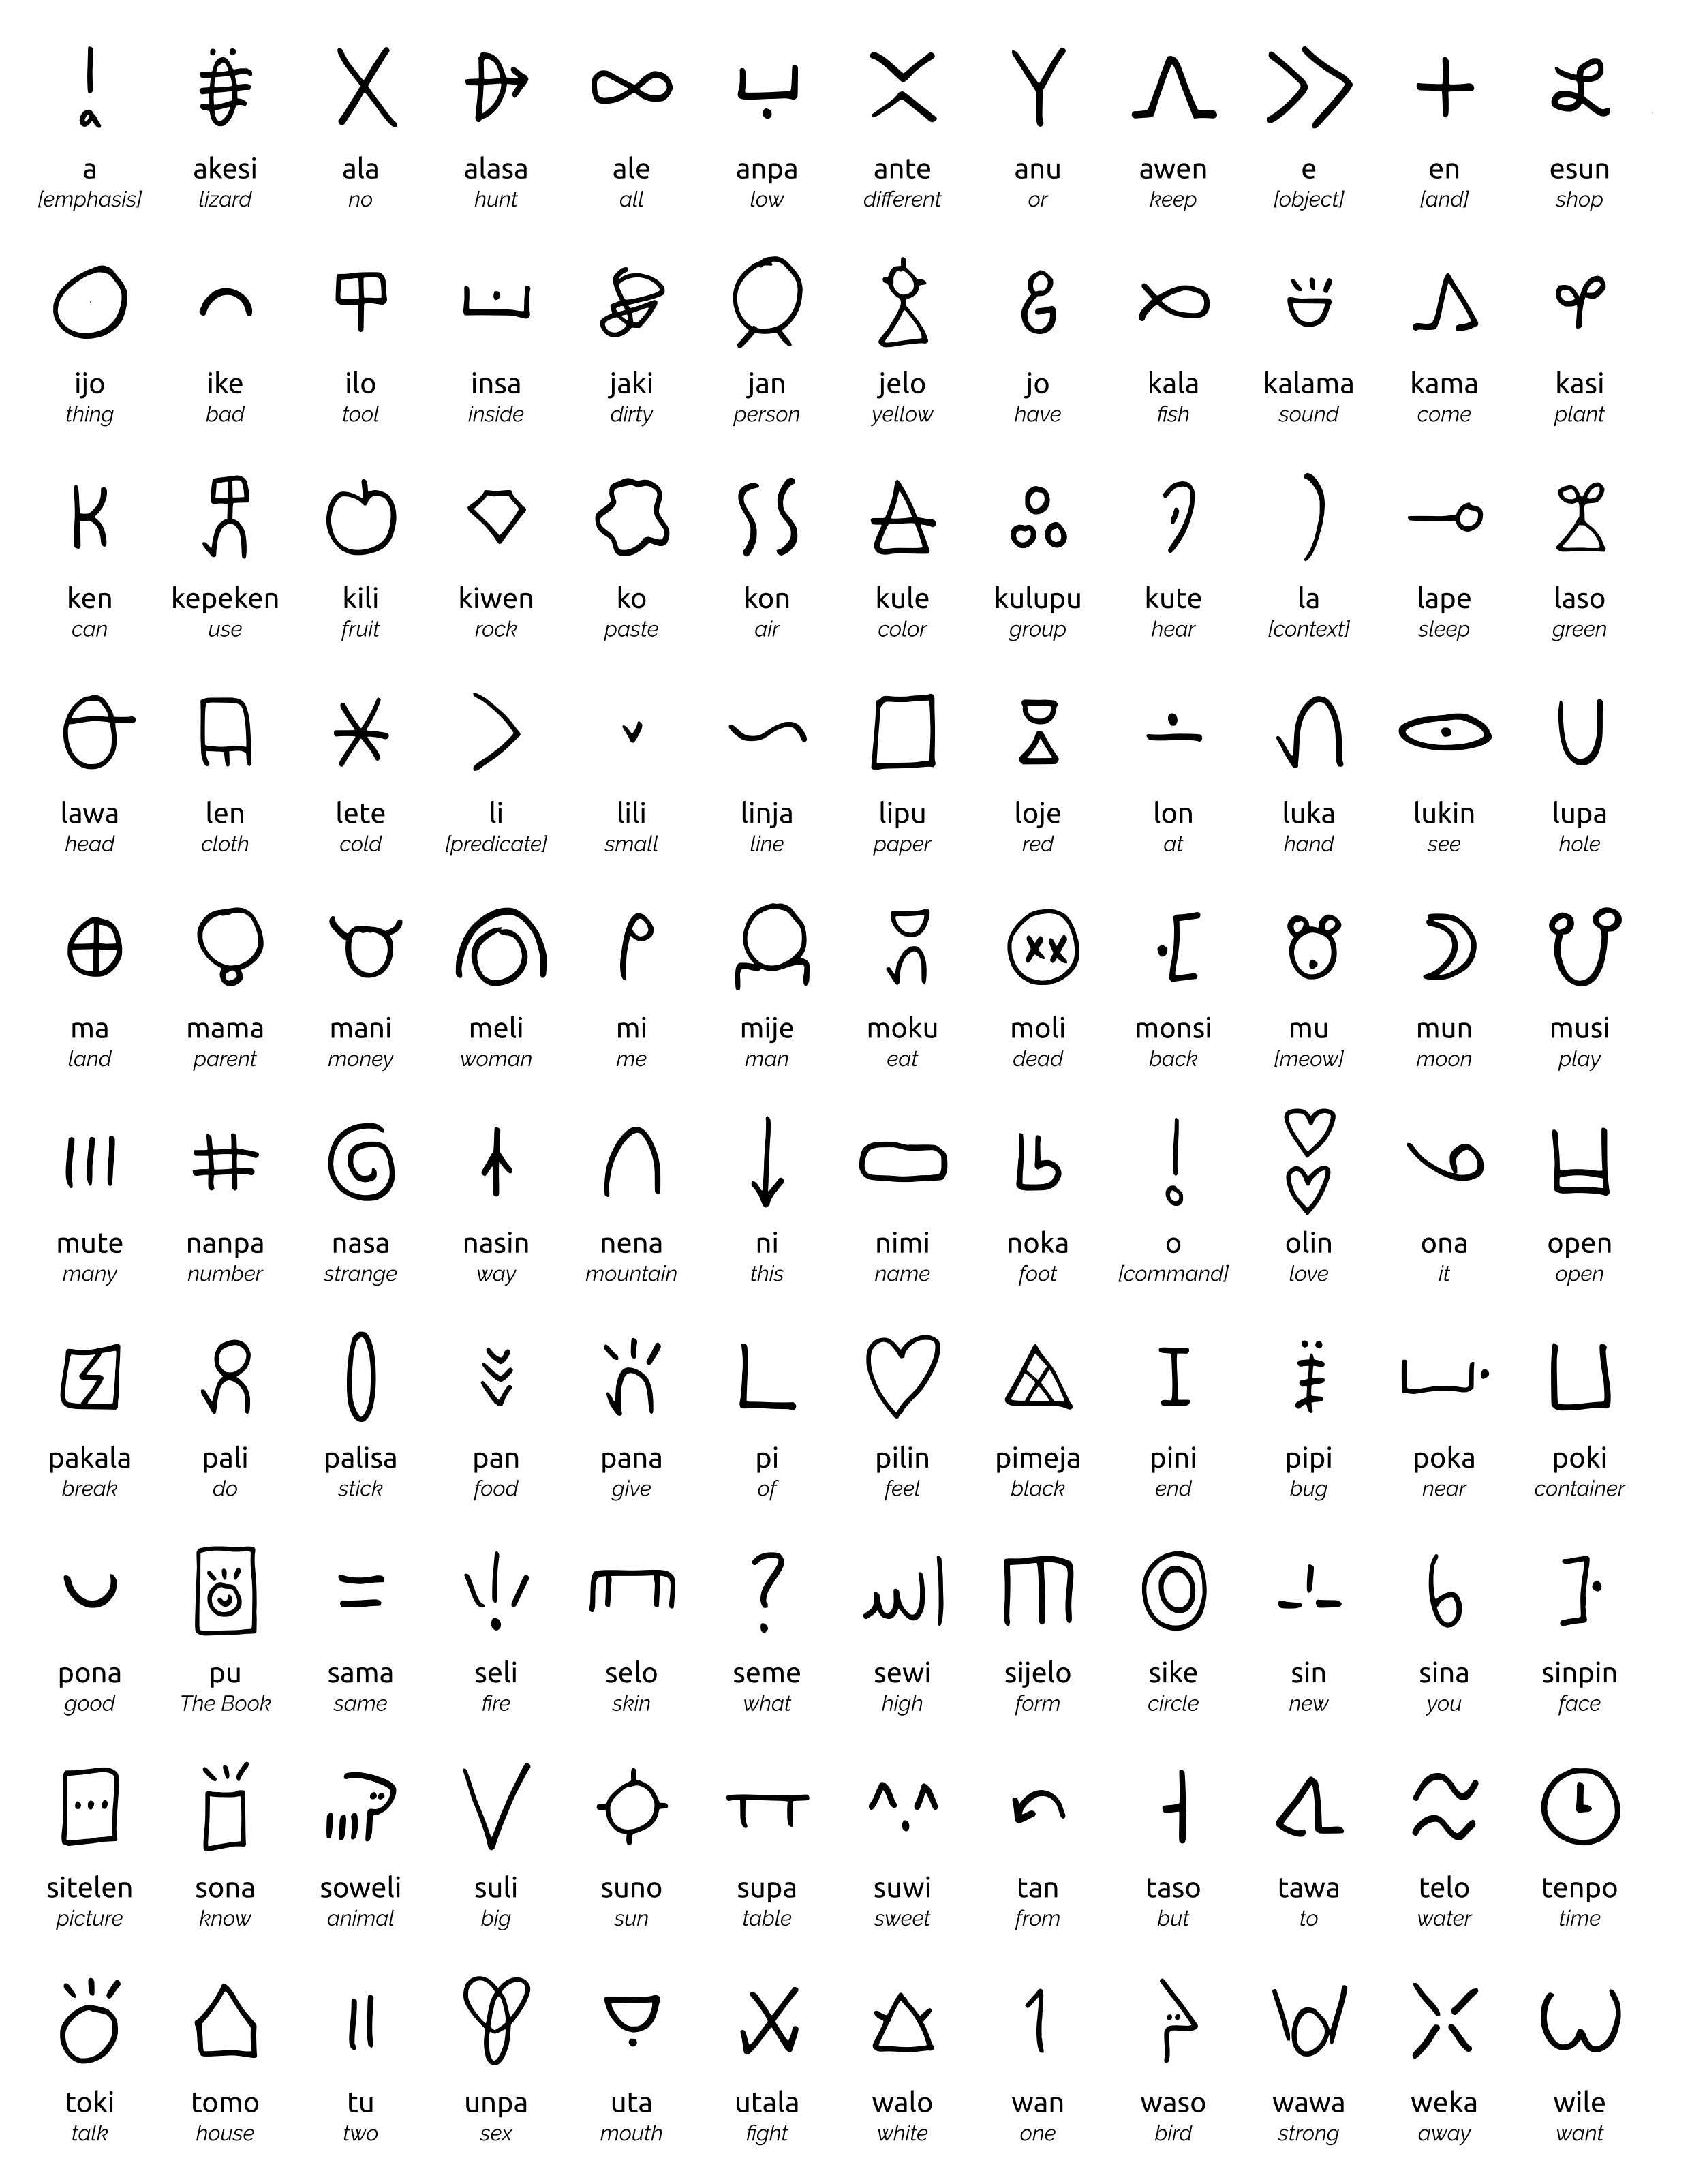
\includegraphics[width=0.95\linewidth]{tokipona.png}

% \begin{tabular}{cccccccc}
% \toprule
% a & akesi & ala & alasa & ale & anpa & ante & anu\\
% (emphasis) & lizard & no & hunt & all & low & different & or\\
% \midrule
% awen & e & en & esun & ijo & ike & ilo & insa\\
% keep & (object) & (and) & shop & thing & bad & tool & inside\\
% \midrule
% jaki & jan & jelo & jo & kala & kalama & kama & kasi\\
% dirty & person & yellow & have & fish & sound & come & plant\\
% \midrule
% ken & kepeken & kili & kiwen & ko & kon & kule & kulupu\\
% can & use & fruit & rock & paste & air & color & group\\
% \midrule
% kute & la & lape & laso & lawa & len & lete & li\\
% hear & (context) & sleep & green & head & cloth & cold & (predicate)\\
% \midrule
% lili & linja & lipu & loje & lon & luka & lukin & lupa\\
% small & line & paper & red & at & hand & see & hole\\
% \midrule
% ma & mama & mani & meli & mi & mije & moku & moli\\
% land & parent & money & woman & me & man & eat & dead\\
% \midrule
% monsi & mu & mun & musi & mute & nanpa & nasa & nasin\\
% back & (meow) & moon & play & many & number & strange & way\\
% \midrule
% nena & ni & nimi & noka & o & olin & ona & open\\
% mountain & this & name & foot & (command) & love & it & open\\
%
% \midrule
% pakala & pali & palisa & pan & pana & pi & pilin & pimeja\\
% break & do & stick & food & give & of & feel & black\\
% \midrule
% pini & pipi & poka & poki & pona & pu & sama & seli\\
% end & bug & near & container & good & book & same & fine\\
%
% \midrule
% selo & seme & sewi & sijelo & sike & sin & sina & sinpin\\
% skin & what & high & form & circle & new & you & face\\
%
% \midrule
% sitelen & sona & soweli & suli & suno & supa & suwi & tan\\
% picture & know & animal & big & sun & table & sweet & from\\
%
% \midrule
% taso & tawa & telo & tenpo & & & & \\
% but & to & water & time & & & & \\
% \bottomrule
% \end{tabular}
\end{center}
\end{document}
